\documentclass[pra,twocolumn,showkeys,preprintnumbers, amsmath,amssymb, aps,A4paper]{revtex4-1}

\usepackage{amsmath}
\usepackage{graphicx}% Include figure files
\usepackage{dcolumn}% Align table columns on decimal point
\usepackage{array}
\usepackage{bm}% bold math
\usepackage{fancyvrb}

\usepackage{amsfonts}
\usepackage{amssymb}
\usepackage{calrsfs}

\usepackage[utf8]{inputenc}
\usepackage{calligra}
\usepackage{calrsfs}
\usepackage[left=2cm,right=2cm,top=2cm,bottom=2cm]{geometry}
\usepackage[mathscr]{euscript}

%\usepackage[left=2cm,right=2cm,top=2cm,bottom=2cm]{geometry}
%\usepackage[mathscr]{euscript}


%\newcommand{\ctu}{\cos(\theta_\uparrow)}



%\preprint{SoftwareX/Elsevier}
\begin{document}

\title{Variational neural network parametrisation of the micromotion operator of periodically driven quantum systems}

\author{German A. Sinuco Leon}
\affiliation{Deparment of Chemistry, Durham University, Durham, United Kingdom.}


\date{\today}
\begin{abstract}
Periodic driving to manipulate the state and properties of a large class of physical systems, solid-state and atomic systems. The descriptoin of periodically driven many-body quantum systems cannot be captured with simple perturbative expansion, and ), and accurate calculation of the time-evolution is required for experimental realisation of dynamical engineering regimes  or robust multquibit gates. Variatoin parametrisation of manybody wave function encode in neural network architectures has been recently introduced succesfuly for compressed representaiont of states with many degrees of freedom. Here we focus on the paramerisation of the Floquet operator of driven two-level systsem using a Restricted Boltzman Machine. We explore the range of strong blue off-resonant driving with strengh varying from weak to strong. The requiured complexity of the RBM with the number of Floquet manifoldand we adapat the to obtain a the Floquet spectrum converges from an approximated solution the Rotating Wave Approximation. The training of the RBM presens all well-known challenges of neural network parametrisation: vanishing gradient.... These results demonstrate explicitly the capabilities and challenges of RBM in describing harmonically driven systems.
\end{abstract}

%\pacs{Valid PACS appear here}% PACS, the Physics and Astronomy
                             % Classification Scheme.
 
\keywords{Periodic driving, Floquet theory, Restricted Boltzman Machine}
\maketitle


\section{\label{sec:Introduction} Introduction}



quantify the expressive power of NN teher is a gap in the understanding .Well understood data sets may offer insight, such as statisticcal physics, manybody physic, tensor networks and renormalisation.


Traininin the machine tmay reveal correlation in the data with physicalmeaning. these larning task.

RBM can paarmetirze complex functions of visible units. 



Wave functinos of many-body systema nd away from equilibrum

RBM representations of topological states


These development raise questions about the expressive powe  of NN for physial problmes. 
can rbm efficiently descrb periodicallly driven dystems. directe relation with exact diagonalisation techniques.


rbm can provide compatct representation for a highly entangled quatum states that does not satisfy the entanblement area., with a number of parameters scaling polynomially with the system size. 


conclussion: general connectino between rbm and tns in arxiv 1701.04831 constitues a brid in usin uch tecniques for harmonically driven systems.

.



In the last decade 
Periodically driven system are almost present in quantum mechanics. both theoreical and experimentally relevant. 
drastica modification of physical systems, including spectral signals \cite{} , 
out-ofpequilibrium states driven by harmonic forces, transformation of states in . Dynamical decoupling with periodic drivings (several harmonics as in the quantum coputing talk I saw), or multiquibe gates by multiple harmonci forces, to floque topological insulators and frequency/time-domain quantum simulations.

The time-evolution operator is key, either to define the time-evolution or for defniniton of effective Hamiltonians. both of them cna be written interms of the Floquet states. Floquet states perturbatoin theory, RWA, Bloch-siegart, ... expansion.... All this approximaiton and general solution are important to uderststand, fore example. 


ML representation of quantum states has been recently very active, showing ... . and compatibility with on-line l earnign and experimental realsiation, in partiuclar for the control of quantums states in quantum computing architectures .... control with floquet.... The reductin of the parametere required, reflection on the ... of the physically accessible states of the Hilbert space, corresponding to very restriced subste, which can be described efffecgively in nothe such as MPS, tensor Netowors.. Such a relatio nbetween ML and ... is currently an active area of research ..

Hrmonically deriven systems can be in the ferquency space has the as a Hubbard model \cite{mine and othres}, and such that time-dependennt problem can be evaluated using toools of static systems \cite{}, which has not been explored sufficiently. Here I study the parametrisation of the Floquet operator using a RBM for the archetypical case of a driven qubit. The RBM is overkilling in this case,with other straight numerical diagonalisaiton of the Floquet Hamiltonian, however it allows to explore the capabilities of, which can be then applied to other more complex systems where exact diagonalisation or cannot be implemented so directly.

The docume is as follows. In Section \ref{sec:FloquetHamiltonian} I present the representation of the time-evlutio operator in terms of Floquet states. In section \ref{sec:RBM}, presents the Restricted Boltzman Machine rerpesentatio of the states and the loss fucntions to evaluate the Floquet spectrum. Section \ref{sec:RBMFloquetStates} shows the representation of Floquet states using the RBM. The central result in presented in section \ref{sec:RBMFloquetSpecttrum}, where I discuss the evalation of the Floquet spectrum (eigenvectors and eigenvalues) evaluated using an RBM parametrisaiton. Discussion of the applcations are presented and conclusion are in sectino...


\begin{figure}
\centering
\caption{\label{fig:SystemSketch} (a) Schematic energy level structure of a generic quantum system. The basis of states consist of a discrete set of energy states, which define several bands according to the level energy spacing. Inter and intra band coupling is induced by electromagnetic radiation tuned at the corresponding frequencies, as indicated by the coupling terms. The wide variety of physical systems described by this model includes (b) trapped ions \cite{PhysRevLett.117.220501}, (c) superconducting qubits \cite{vion2002manipulating} and (d) diamond NV-centres \cite{balasubramanian2009ultralong}.}
\end{figure}


\section{\label{sec:FloquetBloch} Floquet formalism}

Periodically driven quantum systems are described by a Hamiltonian of the form:
\begin{equation}
H(t) = \sum_{i,j}^D E_{i,j} \left| i\right\rangle \left\langle j \right| + \sum_{i,j}^D \sum_{n \in Z} V_{i,j}^{n} e^{i n \omega t} \left| i\right\rangle \left\langle j \right| + \textrm{h.c.}
\label{eq:Hamiltonian}
\end{equation}
where $D$ is the dimension of the Hilbert space, ${E_{i,j}}$ defines the static component of the Hamiltonian, $V_{i,j}^{\ell,n}$ is the coupling between the states $i$ and $j$ oscillating at frequency $n \omega$ (i.e. the $n$-th harmonic of the fundamental frequency $\omega$). 

Solutions to the corresponding Schr\"odinger can be build after finding a priviliged frame of reference where the transformed Hamiltonian is time-independent and diagonal \cite{}. Thus, we are looking for a time-dependent unitary transformation, $U_F(t)$, that satisfies:
\begin{equation}
 U_F^\dagger(t) H(t)  U_F(t) - i \hbar  U_F^\dagger(t) \partial_t  U_F(t) =  \sum_{\bar{i}} \bar{E}_{\bar{i}} \left| \bar{i} \right\rangle \left\langle \bar{i} \right|
\label{eq:Hdressed}
\end{equation}
where $\bar{E}_{\bar{i}}$ with $\bar{i} \in [1,D]$ is the set of eigenstates in the frame of refence where the Hamiltonian is static. In this frame of reference, the time-evolution operator is diagonal and the inverse of $U_F(t)$ can be applied to obtain the time-evolution operator in the original basis. 

Considering the time-dependence of the coupling terms in the Hamiltonian, we parametrise $U_F(t)$ as a Fouries series of the form \cite{ho1983semiclassical}:
\begin{equation}
U_F(t) = \sum_{n\in Z} u_{i,\bar{i}}^{n} e^{-in\omega t} \left| i \right\rangle \left\langle \bar{i} \right|
\label{eq:micromotionexpansion}
\end{equation}

Using this expansion in the transformation rule Eq. (\ref{eq:Hdressed}) and taking into account the orthonormality of the Fourier basis, we obtain the eigenvalue problem:
\begin{eqnarray}
\bar{E}_{\bar{i}}U^{n}_{i,\bar{i}}&=&\sum_{i,j=1}^{D} \sum_{n\in Z}(E_{i,j} - \delta_{i,j} n \hbar \omega)U^{n}_{j,\bar{i}} \nonumber \\
&&+ \sum_{j=1}^D \sum_{m\in Z} \left[ V^{m}_{i,j} U^{n+m}_{j,\bar{i}} + V^{m*}_{ji} U^{m-n}_{j,\bar{i}}\right]
\label{eq:floqueteigenproblem}
\end{eqnarray}
which lead us to a finite matrix representation after truncating the sums in eq. (\ref{eq:micromotionexpansion}). 

For concretness, in this paper we consider a harmonically driven qubit with the Hamiltonian:
\begin{equation}
H = \frac{\hbar \omega_0}{2} \sigma_z + \frac{\hbar \Omega}{2} \sigma_x \cos (\omega t + \phi)
\end{equation}
with the Pauli matrices $\sigma_i$ with $i\in[x,y,z]$ \cite{}.

In this case, the Fourier components of the unitary transformation $U_F(t)$ are the eigenvectors of the matrix:

\begin{widetext}
\begin{equation}
\mathcal{H} = \hbar \omega_0 \begin{pmatrix}
 \frac{1}{2} \sigma_z + 3 \bar{\omega} I & e^{i\phi}\frac{\bar{\Omega}}{4} \sigma_x & 0 & 0 & 0 & 0 &0 \\
 e^{-i\phi}\frac{\bar{\Omega} }{4} \sigma_x &  \frac{1}{2} \sigma_z + 2 \bar{\omega}I & e^{i\phi}\frac{\bar{\Omega}}{4} \sigma_x & 0 & 0 & 0 & 0 \\
0& e^{-i\phi}\frac{\bar{\Omega} }{4} \sigma_x &  \frac{1}{2} \sigma_z + \bar{\omega}I & e^{i\phi}\frac{\bar{\Omega}}{4} \sigma_x & 0 & 0 & 0  \\
0 & 0& e^{-i\phi}\frac{\bar{\Omega} }{4} \sigma_x &  \frac{1}{2} \sigma_z& e^{i\phi}\frac{\bar{\Omega}}{4} \sigma_x & 0 & 0 \\
0 & 0 & 0& e^{-i\phi}\frac{\bar{\Omega} }{4} \sigma_x &  \frac{1}{2} \sigma_z -  \bar{\omega}I & e^{i\phi}\frac{\bar{\Omega}}{4} \sigma_x & 0 \\
0 & 0 & 0 & 0& e^{-i\phi}\frac{\bar{\Omega} }{4} \sigma_x &  \frac{1}{2} \sigma_z - 2 \bar{\omega}I & e^{i\phi}\frac{\bar{\Omega}}{4} \sigma_x   \\
0 & 0 & 0 & 0 & 0& e^{-i\phi}\frac{\bar{\Omega} }{4} \sigma_x &  \frac{1}{2} \sigma_z - 3 \bar{\omega}I 
\end{pmatrix}
\begin{pmatrix}
\frac{1}{2}\\
0 \\
0 \\
0 \\
0 \\
0 \\
0  
\end{pmatrix}
\end{equation}
\end{widetext}

The unitary transformation is of the form.


However, due to the symmetry of the, we can select any set of and. It is natrual to select the central columns and repeat, we have to  parametrise only a reduced set of the elemtnes of the matrix.


In the regime of off-resonant + weak-to-strong driving. More precisely, our numerical results are obtained for the parameters $\omega=1.7 \omega_0$ and the Rabi frequency $\Omega \in [ 0,10 ]\times \omega_0$. Figure presents the energy gap between the dressed states as a function of the Rabi frequency $\Omega$  and the eigen states of selected parameters.  

The wavefunction has the symmetry, $n \rightarrow n+m$,  :
\begin{equation}
U_{i,\bar{i}}^n = U_{i,\bar{i}}^{m+n}
\end{equation}
which is used to reduce the number of paramerter below.

The 

\section{Parametrisation of the micromotion operator}

The dressed states defined by $U_F$ are time-dependent superposition of the elements of the basis:
\begin{equation}
\left| \bar{i} \right\rangle = \sum_{j,n} u^{n}_{j,\bar{i}} e^{i n \omega t}\left|j \right\rangle
\end{equation}
with the coefficientes of $U_F$. 

Following the Troyer Calero ... and tohre, we parametrise theses elements with a pair of Restricted Boltzman Machines (RBM) that define their amplitude and phase. Simple generalisation of the RBM for spin systems. In this case, the state of each cell of the visible layer is given by a set of integers that identify the element .  $\sigma = {j,\bar{i},n}$, the projection of angular momentum of the bare and dressed states, and $n\in Z$ the Floquet manifold index. The state of the hidden layer is $\boldsymbol{h} = (h_1,h_2,h_3,\ldots,h_M)$ with the binary variables $h_i \in {-1,1}$ for $i=1,\ldots M$. 

The micromotion fourier components can be parametrized by:
\begin{equation}
u^{n}_{j,\bar{i}} = \sqrt{\frac{P_{\lambda}(\boldsymbol{\sigma})}{Z}} \exp(\phi_{\mu}(\boldsymbol{\sigma}))
\end{equation}
with the marginal probabilities:
\begin{equation}
P_{\kappa}(\boldsymbol{\sigma}) = \sum_{\{\boldsymbol{h}\}} p_{\kappa}(\boldsymbol{\sigma},\boldsymbol{h})
\end{equation}
obtained from the ... probability.
\begin{equation}
p_{\kappa}(\boldsymbol{\sigma},\boldsymbol{h}) = \exp (\boldsymbol{b}_{\boldsymbol{\sigma}} \cdot \boldsymbol{\sigma} + \boldsymbol{c}_{\boldsymbol{h}} \cdot \boldsymbol{h} + \boldsymbol{h}^T \cdot W_{\boldsymbol{h},\boldsymbol{\sigma}} \cdot \boldsymbol{\sigma})
\end{equation}
for $\kappa={\lambda}$ and $\mu$.

In this case, the symbol $\boldsymbol{\sigma}$ is an array of numbers that 	labels the element of the Floquet matrix. For the driven two level system, we choose $\boldsymbol{\sigma} = i,\bar{i},1/n $, with $i,\bar{i} \in {-1/2,1/2}$ the projection of angular momentum of the bare and dressed states, and $n\in Z$ the Floquet manifold index.

The single layer RBM allows us to obtain an analytical expression for the marginal probabilities:
\begin{equation}
P_{\kappa}(\boldsymbol{\sigma}) = \exp(\boldsymbol{b}_{\boldsymbol{\sigma}}\cdot\boldsymbol{\sigma}) \prod_{j=1}^{h} \cosh(\boldsymbol{c}_j+ \boldsymbol{W}_j\cdot\boldsymbol{\sigma})
\end{equation}

The cost function can be build from our objective of diagonaliing the matrix. We define the distance of matrix from a diagonal form ...
\begin{equation}
\left\|\mathcal{L}\right\| = \sum_{i} \left| \sum_{j} |\mathcal{H}_{j,i}| - |\mathcal{H}_{i,i}| \right|^{2}
\end{equation}
which is sum of the square of differences between the element of the diagonal and the sum of the norms along each column of the transformed Hamiltonian. 

The parameters are then 


\section{\label{sec:RBMFloquetStates} RBM parametrisation of Floquet states} 

As a first test of the power of representation of the RBM, we evaluate the of the micromotion operator evaluated numerically. This is done by diagonalising the matrix Eq. (\ref{}) and selecting the central group of dressed states.

Since the micromotion opertor can be interpretated as the amplitued of probability in the extended Floquet basis, we adjust the parameters $\boldsymbol{b}, \boldsymbol{h}, \boldsymbol{W} $ using the Kull-lll loss function:
\begin{equation}
k = \sum_i p_i \log \frac{p_i}{p_i}
\end{equation}
with $p_i = |u_{j,i}|^2$

The training starts of wit a random distribution of all parameters with choosen as ..to train both RBm parametrisation of the amplitude and the phase, I loop swapping one after the other, starting of a random initiailization of the RBM parameters. The parameers of the amplitude are choosen as randon, while 

Typical training problems and parameters. Accuracy. 


\begin{figure*}
\centering
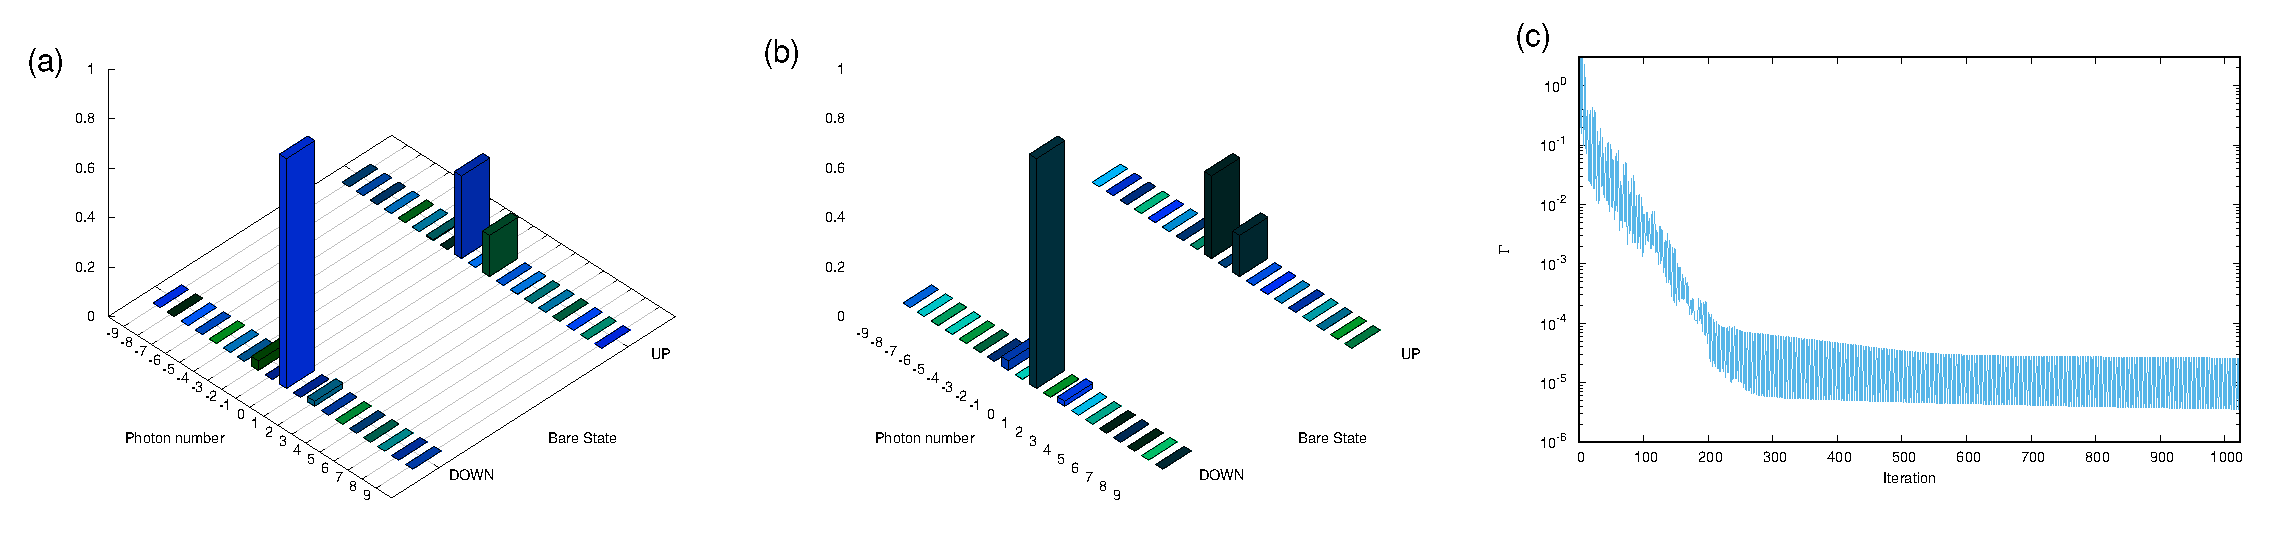
\includegraphics[width=\textwidth]{FloquetvsRBM_Floquet1st.eps}
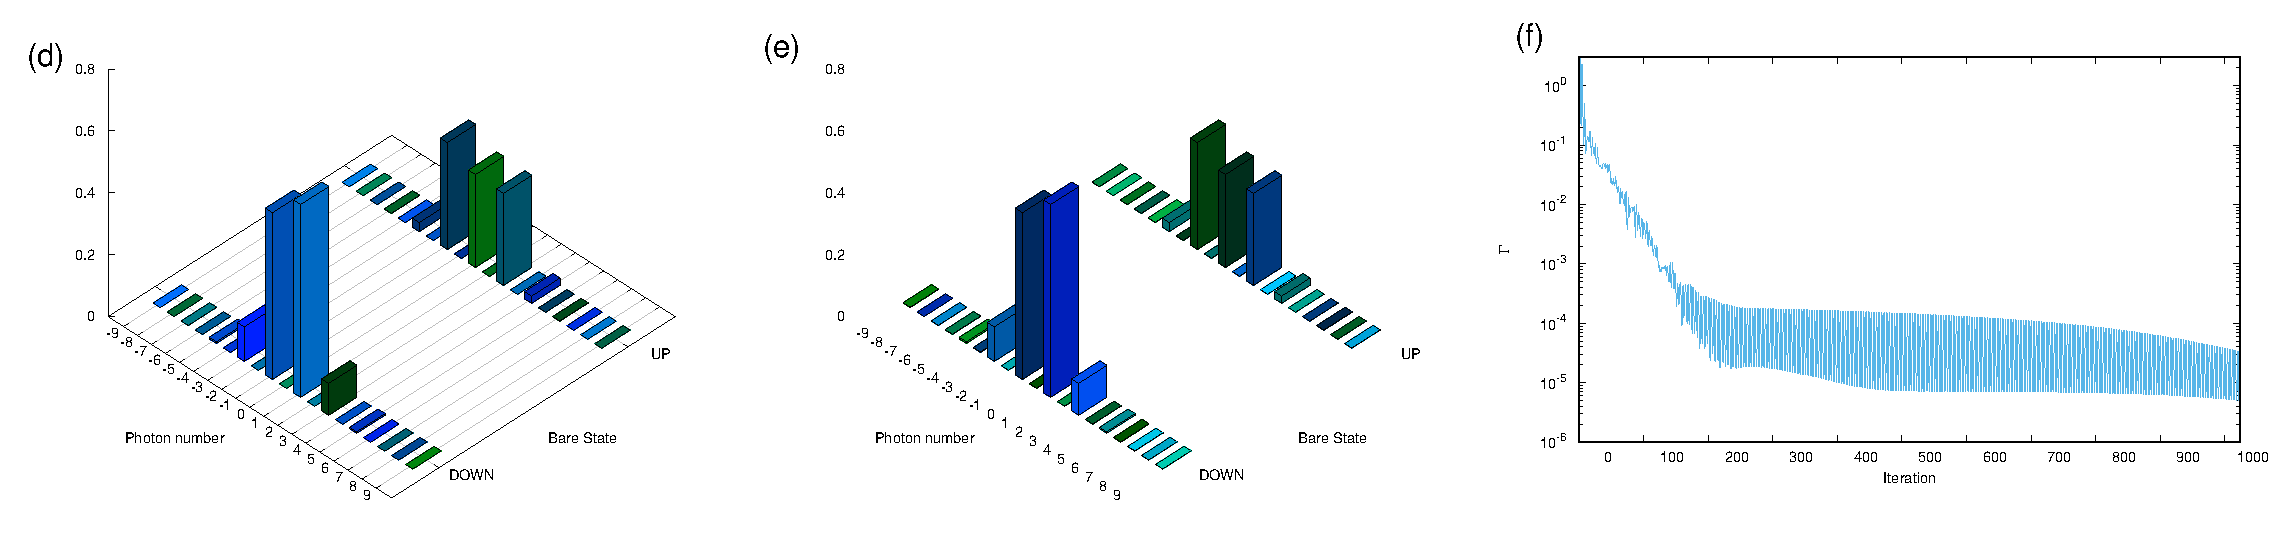
\includegraphics[width=\textwidth]{FloquetvsRBM_Floquet2nd.eps}
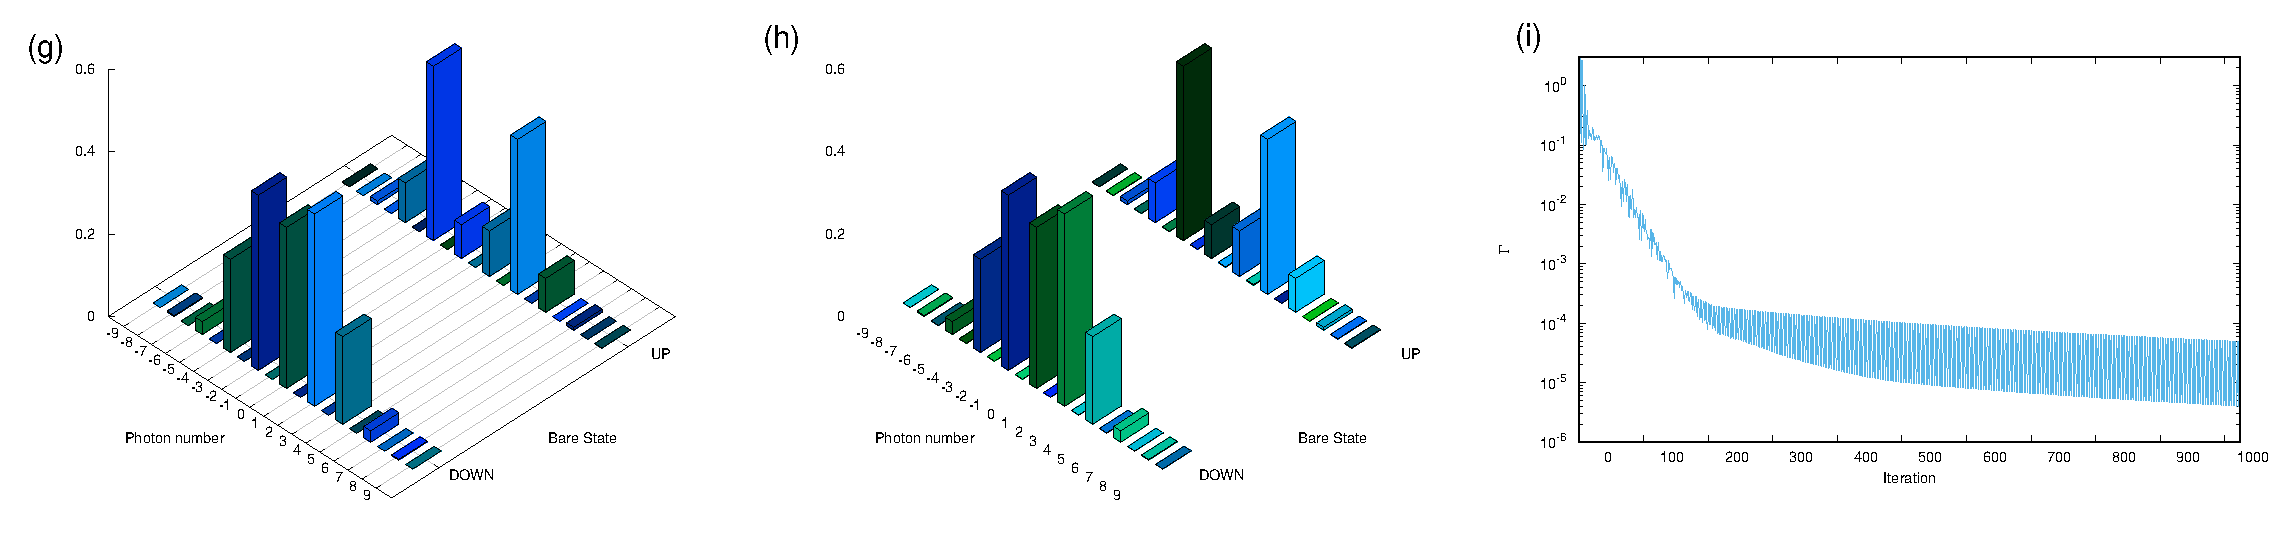
\includegraphics[width=\textwidth]{FloquetvsRBM_Floquet3rd.eps}
\caption{\label{fig:FloquetFitRBM} Wavefunction of floquet states in the expanded space corresponding to the coefficients $u^{n}_{i,h}$ in Eq. (). The column on the left (panels (a),(d) and (e)) show the mangiuted and phase of the fitted wave funciton with the RBM. For comparison, the panels in the central column ((b),(e) and (h)) wshow the numerically exact calculation . The column on the right . In all cases we consider a two-level system driven by a frequency annd with strenght $\Omega=$, corresponding to the first, second and last rows, respectively}
\end{figure*}


\section{\label{sec:RBMFloquetSpectrum} Floquet spectrum and micromotion}

Finding the full spectrum of quasienergies and the .

As an initial guess for the parameters, we train the RBM to fit the RWA, which can be evluated in . The second is the definition of a loss fucntion. IN this case we wnat a that the matrix ooperion... lead to a diagnonal form .we define distance as the difference between the of the values with the correponding diagonal elelmemtn. The training of this ..  shown in ...

As a second form of the loss function is a quantification of the diffenece between the lefhs vectors and the initila vectors. They should only differr in the scale, such . the candidate eigenvalue is chooslen as teh ratio between ... and .... Then we evaluate the difference.  The traiing .. suffer similar difficulties taking a long number of steps and requrieing a small loss rate. 


Combination of the two loss functions during traingin in a randomly between loss functions. We observe a spped up of the traiing, improve of the fidelity with the esxac, as well an improvment of the numerically exact Floquet spectrum.


\begin{figure}
\centering
\includegraphics[width=0.5\textwidth]{EnergyError.eps}
\includegraphics[width=0.5\textwidth]{Fidelity.eps}
\includegraphics[width=0.5\textwidth]{LossInitFinal.eps}
\caption{\label{fig:MicromotionResults} Ensemble average of the RBM performance to fit the micromotion operator of a driven qubit as function of the driving amplitude. (a) The average error in the energy computation (b) Average fidelity of the RBM parametrized dressed states with respect to the numerically exact Floquet states. (c) Initial and final values of the loss function $\Gamma$ defined in . The points represent average over 24 .. of the RBM, with the bars the standard deviation. }
\end{figure}


\section{\label{sec:discussion} Discussion}

Loss function with slow learning. Investigation in better loss function as well as dragging tools from ML to speep up .. 

The difficutly of training consittues a tool for charactersing physicsl system as ... . Hre we have observed that complex wavefuntion rquire more traiing effort. application for example to floque driven systems.

Applicaton for evaluating the longtime evluation. nitial guess functions to improve convegencey. COnversely, the training wave functin and the distribution/correlation of the coefficients correlated with othe critier of the system..

The application of symmetries an boundary coditions to the floquet states. Also, this can be readly extended to multimode scaling of multimodedriven system (with unconmensurable frequencies).
 


RBM parametrisation fits any function.

Floquet states requiring more Fourier components are harder to train.

several ways to define a loss function.

Slow gradident

random selection of criteria similar to ensemble learning

the RWA approximation is a good start generically and evolvs towards the solution. sppeding up the  convergence ML .

More interesting is the constuction of the iniital guess and restriction of the solutions explored, for example that the amplitude of Floquet manifolds should be small.

here we explored the RBM parametrisation to build the micromotion operator. Other parameteisation  can be more efficient for optimisation. Such construction of the initial guess and constrains can be come from using Tensor Networks parametrisation, or ... 


\section{Conclussion}
In this paper we present a premier explorative study of the use of RBM for the parametriation of Floquet operators, in an archetypical periodically driven system. We obtain that trining of the can be done , which is equivalent to the experimentally demonstrated in .. .with online learning of the wavefunction.

The evaluation of the Floquet spectrum is a mor difficult task. he initial guess guides the minimun of th e defined loss function. simple definitos vse on the prpertis of a diaognal matris and present low grdients .  combination of loss funciton sa better, reflection on the ensemble learning combination fo other simple archigecture of the wave fucntion, eg a NN can led to for more comple systems tahtn the studeid here. 

In this work we present a initial exploration of using RBM for Floqeut problems. the Floquet states staes can be parametrised efficiently following similar approches, even with an altenative fitting of the complex and the wavefunction amplitude. this task can be qualified as easy, rapid from random distributon. 

Finding the Floquet sates is a harder task. using as initial guess the RWA training . the function has a slow after a fast decline. however a combination of loss funcitons satisfied by any dagnonal matrix  or the eigne vectors helps to guide the search. configuraiotn.. . Perhaps a different . The micromotion operator is the time-evolution operator, then other ML architehqure mighth present better. Also

This starting point for exploratioon of the use of parametrisatio for more complex ...like .. .  The numerical effor for the case studied here is overkilling, however we explore typical taht might be present in other driven quantum systems. 



\bibliography{LibraryBib}


\section*{Acknowledgements}
We acknowledge fruitful comments and input from Dr. Juan Sebastian Totero Gongora. This work has been supported by the University of Sussex.

\section*{Appendix A: Restriced Boltzman Machine parametrisation of $u^n_{j,\bar{i}}$}
\section*{Appendix B: Typical and no so typical training results}
\section*{Appendix A: Typical example of the matrix representation of the multimode Hamiltonian}

\end{document}
